%%%%%%%%%%%%%%%%%%%%%%%%%%%%%%%%%%%%%%%%%
% Beamer Presentation
% LaTeX Template
% Version 1.0 (10/11/12)
%
% This template has been downloaded from:
% http://www.LaTeXTemplates.com
%
% License:
% CC BY-NC-SA 3.0 (http://creativecommons.org/licenses/by-nc-sa/3.0/)
%
%%%%%%%%%%%%%%%%%%%%%%%%%%%%%%%%%%%%%%%%%

%----------------------------------------------------------------------------------------
%	PACKAGES AND THEMES
%----------------------------------------------------------------------------------------

\documentclass{beamer}
\setbeamertemplate{navigation symbols}{} % comment this out to ADD navigation tools

\usepackage{sansmathaccent}
\pdfmapfile{+sansmathaccent.map}

\mode<presentation> {

% The Beamer class comes with a number of default slide themes
% which change the colors and layouts of slides. Below this is a list
% of all the themes, uncomment each in turn to see what they look like.

%\usetheme{default}
%\usetheme{AnnArbor}
%\usetheme{Antibes}
%\usetheme{Bergen}
%\usetheme{Berkeley}
%\usetheme{Berlin}
%\usetheme{Boadilla}
%\usetheme{CambridgeUS}
%\usetheme{Copenhagen}
%\usetheme{Darmstadt}
%\usetheme{Dresden}
%\usetheme{Frankfurt}
%\usetheme{Goettingen}
%\usetheme{Hannover}
%\usetheme{Ilmenau}
%\usetheme{JuanLesPins}
%\usetheme{Luebeck}
%\usetheme{Madrid}
%\usetheme{Malmoe}
%\usetheme{Marburg}
%\usetheme{Montpellier}
%\usetheme{PaloAlto}
%\usetheme{Pittsburgh}
%\usetheme{Rochester}
%\usetheme{Singapore}
\usetheme{Szeged}
%\usetheme{Warsaw}

% As well as themes, the Beamer class has a number of color themes
% for any slide theme. Uncomment each of these in turn to see how it
% changes the colors of your current slide theme.

%\usecolortheme{albatross}
\usecolortheme{beaver}
%\usecolortheme{beetle}
%\usecolortheme{crane}
%\usecolortheme{dolphin}
%\usecolortheme{dove}
%\usecolortheme{fly}
%\usecolortheme{lily}
%\usecolortheme{orchid}
%\usecolortheme{rose}
%\usecolortheme{seagull}
%\usecolortheme{seahorse}
%\usecolortheme{whale}
%\usecolortheme{wolverine}

%\setbeamertemplate{footline} % To remove the footer line in all slides uncomment this line
%\setbeamertemplate{footline}[page number] % To replace the footer line in all slides with a simple slide count uncomment this line

%\setbeamertemplate{navigation symbols}{} % To remove the navigation symbols from the bottom of all slides uncomment this line
}

\usepackage{graphicx} % Allows including images
\usepackage{booktabs} % Allows the use of \toprule, \midrule and \bottomrule in tables
\usepackage{amssymb}
\usepackage{amsmath}
\usepackage{array}
\usepackage{longtable}
\usepackage{everysel}
\usepackage{xtab}
\usepackage{ragged2e}
\usepackage[labelfont=bf]{caption}
\usepackage{url}
\usepackage{datetime}
\usepackage{setspace}
\usepackage{multicol}
\usepackage{vwcol}

% texpos setup for placing text or images anywhere on the page
\usepackage[absolute,overlay]{textpos}
\setlength{\TPHorizModule}{30mm}
\setlength{\TPVertModule}{\TPHorizModule}
\textblockorigin{10mm}{10mm} % start everything near the top-left corner

% line spacing options
%\singlespacing
%\onehalfspacing
%\doublespacing
\setstretch{1.3} % for custom spacing


%---------------------------------------------------------------------------
%	TITLE PAGE
%---------------------------------------------------------------------------

\title[Flexible and Efficient Data Flow for MapReduce]{Flexible and Efficient \\ Data Flow for MapReduce} % The short title appears at the bottom of every slide, the full title is only on the title page

\author{Adam Martini} % your name
\institute[UO] % Your institution as it will appear on the bottom of every slide, may be shorthand to save space
{
University of Oregon \\ % Your institution for the title page
\medskip
\textit{martini@cs.uoregon.edu} % Your email address
}

\newdate{date}{5}{6}{2014}
\date{\displaydate{date}} % Date, can be changed to a custom date

\begin{document}

\begin{frame}
\titlepage % Print the title page as the first slide
\end{frame}

%\begin{frame}
%\frametitle{Overview} % Table of contents slide, comment this block out to remove it
%\tableofcontents % Throughout your presentation, if you choose to use \section{} and \subsection{} commands, these will automatically be printed on this slide as an overview of your presentation
%\end{frame}

%I suggest that you focus on the main points including the following:
%- what is the context of your work and why it is important? (one slide)
%
%- what are the key questions that you are exploring in your paper? (one slide)
%
%- what is the method/approach you used to organize selected studies (i.e. what are the 
%main aspects/metrics/issues you chose to compare and contrast different approaches, 
%in short what criteria you use to organize prior approaches in your report)
%is this your own method or you borrowed it from other places? (one slide)
%
%- What are the main points, findings, lessons learned in an organized (point by point) manner,
%again did you drive these points yourself or they are stated in other studies? (a few slides)

%----------------------------------------------------------------------------------------
%	PRESENTATION SLIDES
%----------------------------------------------------------------------------------------

%------------------------------------------------
%\section{Introduction} % Sections can be created in order to organize your presentation into discrete blocks, all sections and subsections are automatically printed in the table of contents as an overview of the talk
%------------------------------------------------

\section{Background} % A subsection can be created just before a set of slides with a common theme to further break down your presentation into chunks
% 1

\begin{frame}

\begin{textblock}{2.4}[0.5,0.5](4,0.525)

\includegraphics[scale=.3]{hadoop.jpeg}
\end{textblock}

\begin{textblock}{2.4}[0.5,-.65](4,0.525)

\includegraphics[scale=.3]{pigpen.jpeg}
\end{textblock}

\begin{textblock}{2.4}[0.5,-1.3](4,0.525)

\includegraphics[scale=.25]{hive.png}
\end{textblock}

\begin{minipage}{7.8cm}

\begin{itemize}
\item What is MapReduce?
	\begin{itemize}
	\item A framework popularized by Google circa 2004
	\item Provides transparent scalability and fault tolerance for ``embarrassingly parallel'' tasks
	\end{itemize}
\item Why do we need it? 
	\begin{itemize}
	\item Initially designed to solve PageRank scalability issues
	\item Big Data is everywhere!
	\item Non-parallel programming experts need a way to efficiently manipulate very large datasets
	\end{itemize}
\end{itemize}
\end{minipage}

\end{frame}


\begin{frame}{Strengths}

\begin{textblock}{5}[0.5,-.31](4,0.525)
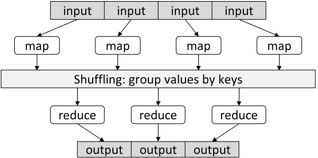
\includegraphics[scale=.6]{mapreduce.jpeg}
\end{textblock}

\begin{minipage}{4cm}
\begin{enumerate}[1)]
\item Massively scalable
\item Can operate on commodity hardware
\item Transparency:
	\begin{itemize}
	\item Data locality
	\item Fault tolerance
	\end{itemize}
\end{enumerate}
\end{minipage}

\end{frame}


\begin{frame}{Weaknessess}

\begin{itemize}
\item Flexibility
	\begin{itemize}
	\item Data flow (and algorithm design) is forced to conform to an oversimplified computational model
	\end{itemize}
\item Efficiency (wrt Data Flow)
	\begin{itemize}
	\item Programs handle data non-optimally $\Rightarrow$ performance loss
	\end{itemize}
\item Take Away
	\begin{itemize}
	\item Improved flexibility can improve efficiency, but the inverse does not hold
	\item \textbf{Focus on performance gains leads to a wide variety of application specific MapReduce derivatives}
	\end{itemize}
\end{itemize}

\end{frame}

\section{Main Points}

\begin{frame}{Data Flow Improvements}

\begin{textblock}{4.2}[0.5,-.5](4,0.525)

\includegraphics[scale=.5]{bigdata.jpeg}
\end{textblock}

Extensions to existing frameworks focus on more flexible work flow, while new frameworks for specific applications focus on improved data flow.\\
\vspace{.5cm}
\textbf{3 Main Directions:}
\begin{itemize}
\item Iterative MapReduce
\item Graph Dependent Models
\item Time Aware Models
\end{itemize}

\end{frame}

\begin{frame}{Iterative MapReduce}

\begin{textblock}{4}[0.5,-.6](4,0.525)
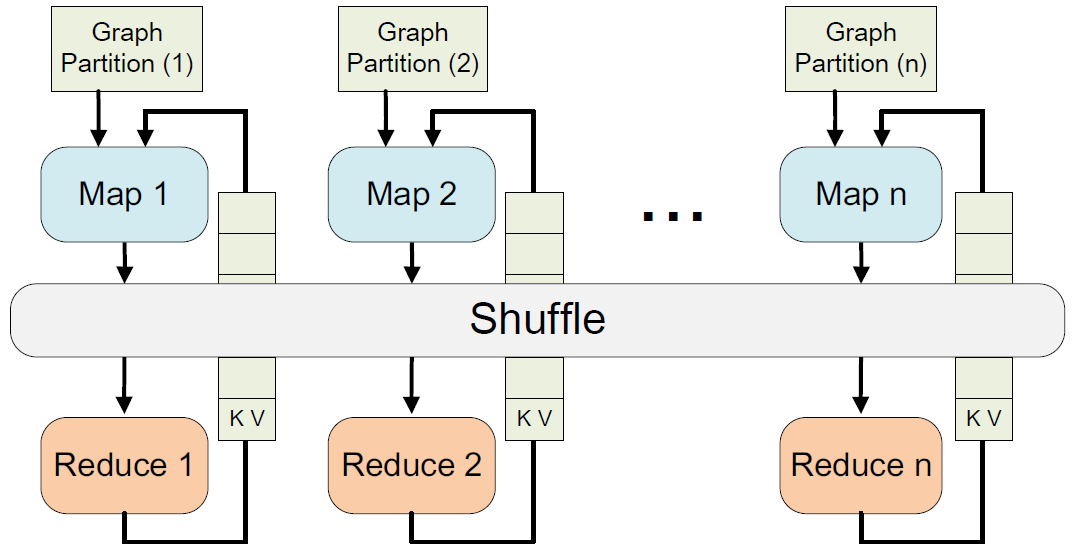
\includegraphics[scale=.18]{iterprocess.png}
\end{textblock}

Primarily inspired by Machine Learning applications that iteratively update a set of dynamic variables using a set of static data instances.\\
\vspace{.5cm}
\textbf{Why}
\begin{itemize}
\item Data IO is slow!
\end{itemize}
\textbf{How}
\begin{itemize}
\item Hold invariant data in memory
\item Hold reductions in memory for convergence checking
\end{itemize}

\end{frame}

\begin{frame}{Iterative MapReduce: Frameworks}

\begin{itemize}
\item \textbf{Spark} -- A very popular framework that supports lazy evaluation, efficient fault tolerance, and iterative machine learning tasks... much faster than Hadoop!
\item \textbf{HaLoop} -- The first framework to introduce convergence checking data optimizations
\item \textbf{Twister} -- Iterative MapReduce with an optional combine step before reduction (also available in Hadoop)
\item \textbf{Shredder/Incoop} -- A GPU accelerated iterative MapReduce framework with an intelligent data chunking algorithms
\end{itemize}

\end{frame}


\begin{frame}{Graph Dependent Models}
\textbf{Two Flavors} -- Frameworks built to support graph updates (PageRank), and frameworks that build data flow DAG's from execution requests.  Both flavors rely on graph structure for optimization.\\
\vspace{.1cm}
\textbf{Why}
\begin{itemize}
\item Graphs contain information about dependencies!
\end{itemize}
\textbf{How}
\begin{itemize}
\item Limit computation based on need
\item Recognize potential for optimization based on structure (cycles, vertical and horizontal fusion)
\end{itemize}

\end{frame}

\begin{frame}{Graph Dependent Models: Frameworks}

\begin{itemize}
\item \textbf{Percolator} -- Developed by Google to replace MapReduce.  Updates only a portion of PageRank indices by propagating the influence of new, or altered, web pages.
\item \textbf{Pregel} -- A general framework for superstep-based graphical updates.  Allows for dynamic changes to graph structure.
\item \textbf{Ceil} -- Uses runtime analysis of dependency graphs to dynamically optimize execution.  Runtime analysis allows for detection of iterative/recursive patterns.
\item \textbf{Flumejava} -- Preprocesses execution plan to generate a DAG, which is used to perform fusion-based optimizations.
\end{itemize}

\end{frame}


\begin{frame}{Time Aware Models}
Time aware models use logical timestamps in conjunction with graphical data flow models to achieve greater flexibility in program design, while reducing computational latency.\\
\vspace{.1cm}
\textbf{Why}
\begin{itemize}
\item More flexible program design eliminates the need to combine several application specific frameworks
\end{itemize}
\textbf{How}
\begin{itemize}
\item More expressive language to define complex parallel patterns
\item A communication transparency layer to provide automated event coordination
\end{itemize}

\end{frame}

\begin{frame}{Graph Dependent Models: Frameworks}

\begin{itemize}
\item \textbf{Naiad} -- Represents computation using a graph with \emph{stateful} nodes that are capable of sending data flow messages without global coordination.  Asynchronous events are coordinated by providing a guarantee that messages will be delivered at a given time, or that the system will be capable of delivering a message by a given time.  The results is a system that outperforms popular frameworks in their target domain.
\end{itemize}

\end{frame}


\section{Conclusion}

\begin{frame}{Take Away}

\begin{textblock}{3.7}[0.5,-.28](4,0.525)
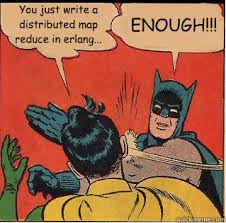
\includegraphics[scale=.6]{batman.jpeg}
\end{textblock}

\begin{minipage}{6.5cm}
\begin{itemize}
\item MapReduce is a simple model that provides useful transparency, but it was not meant to do everything!
\item With increased flexibility comes programmer responsibility...
\item \textbf{The Ultimate Goal}\\
A single framework that provides transparent scalability/fault tolerance, a friendly interface, automatic optimization, and expressivity.
\end{itemize}
\end{minipage}

\end{frame}







%------------------------------------------------

\section{References}

\begin{frame}[allowframebreaks]{References}
\footnotesize{
\begin{thebibliography}{1}

\bibitem{mapreduce}
Jeffrey Dean and Sanjay Ghemawat,
\newblock ``Mapreduce: simplified data processing on large clusters,''
\newblock {\em Communications of the ACM}, vol. 51, no. 1, pp. 107--113, 2008.

\bibitem{survey}
Kyong-Ha Lee, Yoon-Joon Lee, Hyunsik Choi, Yon~Dohn Chung, and Bongki Moon,
\newblock ``Parallel data processing with mapreduce: a survey,''
\newblock {\em AcM sIGMoD Record}, vol. 40, no. 4, pp. 11--20, 2012.

\bibitem{spark}
Matei Zaharia, Mosharaf Chowdhury, Tathagata Das, Ankur Dave, Justin Ma, Murphy
  McCauley, Michael~J Franklin, Scott Shenker, and Ion Stoica,
\newblock ``Resilient distributed datasets: A fault-tolerant abstraction for
  in-memory cluster computing,''
\newblock in {\em Proceedings of the 9th USENIX conference on Networked Systems
  Design and Implementation}. USENIX Association, 2012, pp. 2--2.

\bibitem{pregel}
Grzegorz Malewicz, Matthew~H Austern, Aart~JC Bik, James~C Dehnert, Ilan Horn,
  Naty Leiser, and Grzegorz Czajkowski,
\newblock ``Pregel: a system for large-scale graph processing,''
\newblock in {\em Proceedings of the 2010 ACM SIGMOD International Conference
  on Management of data}. ACM, 2010, pp. 135--146.

\bibitem{flumejava}
Craig Chambers, Ashish Raniwala, Frances Perry, Stephen Adams, Robert~R Henry,
  Robert Bradshaw, and Nathan Weizenbaum,
\newblock ``Flumejava: easy, efficient data-parallel pipelines,''
\newblock in {\em ACM Sigplan Notices}. ACM, 2010, vol.~45, pp. 363--375.

\bibitem{naiad}
Derek~G Murray, Frank McSherry, Rebecca Isaacs, Michael Isard, Paul Barham, and
  Martin Abadi,
\newblock ``Naiad: a timely dataflow system,''
\newblock in {\em Proceedings of the Twenty-Fourth ACM Symposium on Operating
  Systems Principles}. ACM, 2013, pp. 439--455.

\bibitem{nectar}
Pradeep~Kumar Gunda, Lenin Ravindranath, Chandramohan~A Thekkath, Yuan Yu, and
  Li~Zhuang,
\newblock ``Nectar: Automatic management of data and computation in
  datacenters.,''
\newblock in {\em OSDI}, 2010, pp. 75--88.


\end{thebibliography}
}
\end{frame}

%------------------------------------------------

\begin{frame}
\Huge{\centerline{The End}}
\end{frame}

%---------------------------------------------------------------------------------------

%\begin{frame}[allowframebreaks]{References}
%\begin{small}
%\bibliographystyle{plainnat}
%\bibliography{references}
%\end{small}
%\end{frame}

\end{document} 